\let\negmedspace\undefined
\let\negthickspace\undefined
\def\inputGnumericTable{}  
\documentclass[journal,12pt,onecolumn]{IEEEtran}
\usepackage{cite}
\usepackage{amsmath,amssymb,amsfonts,amsthm}
\usepackage{algorithmic}
\usepackage{graphicx}
\usepackage{textcomp}
\usepackage{xcolor}
\usepackage{txfonts}
\usepackage{listings}
\usepackage{enumitem}
\usepackage{mathtools}
\usepackage{gensymb}
\usepackage[breaklinks=true]{hyperref}
\usepackage{tkz-euclide} % loads  TikZ and tkz-base
\usepackage{listings}
\usepackage[latin1]{inputenc}                                 
\usepackage{color}    
\usepackage{gvv}                       
\usepackage{array}                                            
\usepackage{longtable}                                        
\usepackage{calc}                                             
\usepackage{multirow}                                         
\usepackage{hhline}                                           
\usepackage{ifthen}                                           
\usepackage{lscape}  
%
%\usepackage{setspace}
%\usepackage{gensymb}
%\doublespacing
%\singlespacing

%\usepackage{graphicx}
%\usepackage{amssymb}
%\usepackage{relsize}
%\usepackage[cmex10]{amsmath}
%\usepackage{amsthm}
%\interdisplaylinepenalty=2500
%\savesymbol{iint}
%\usepackage{txfonts}
%\restoresymbol{TXF}{iint}
%\usepackage{wasysym}
%\usepackage{amsthm}
%\usepackage{iithtlc}
%\usepackage{mathrsfs}
%\usepackage{txfonts}
%\usepackage{stfloats}
%\usepackage{bm}
%\usepackage{cite}
%\usepackage{cases}
%\usepackage{subfig}
%\usepackage{xtab}
%\usepackage{longtable}
%\usepackage{multirow}
%\usepackage{algorithm}
%\usepackage{algpseudocode}
%\usepackage{enumitem}
%\usepackage{mathtools}
%\usepackage{tikz}
%\usepackage{circuitikz}
%\usepackage{verbatim}
%\usepackage{tfrupee}
%\usepackage{stmaryrd}
%\usetkzobj{all}
%    \usepackage{color}                                            %%
%    \usepackage{array}                                            %%
%    \usepackage{longtable}                                        %%
%    \usepackage{calc}                                             %%
%    \usepackage{multirow}                                         %%
%    \usepackage{hhline}                                           %%
%    \usepackage{ifthen}                                           %%
  %optionally (for landscape tables embedded in another document): %%
%    \usepackage{lscape}     
%\usepackage{multicol}
%\usepackage{chngcntr}
%\usepackage{enumerate}

%\usepackage{wasysym}
%\documentclass[conference]{IEEEtran}
%\IEEEoverridecommandlockouts
% The preceding line is only needed to identify funding in the first footnote. If that is unneeded, please comment it out.

\newtheorem{theorem}{Theorem}[section]
\newtheorem{problem}{Problem}
\newtheorem{proposition}{Proposition}[section]
\newtheorem{lemma}{Lemma}[section]
\newtheorem{corollary}[theorem]{Corollary}
\newtheorem{example}{Example}[section]
\newtheorem{definition}[problem]{Definition}
%\newtheorem{thm}{Theorem}[section] 
%\newtheorem{defn}[thm]{Definition}
%\newtheorem{algorithm}{Algorithm}[section]
%\newtheorem{cor}{Corollary}
\newcommand{\BEQA}{\begin{eqnarray}}
\newcommand{\EEQA}{\end{eqnarray}}
\newcommand{\define}{\stackrel{\triangle}{=}}
\theoremstyle{remark}
\newtheorem{rem}{Remark}

%\bibliographystyle{ieeetr}
\begin{document}
%

\bibliographystyle{IEEEtran}


\vspace{3cm}

\title{
%	\logo{
Experiment-8

\large{EE:2801 DSP-Lab}

Indian Institute of Technology, Hyderabad
%	}
}
\author{Jay Vikrant

EE22BTECH11025
}	


% paper title
% can use linebreaks \\ within to get better formatting as desired
%\title{Matrix Analysis through Octave}
%
%
% author names and IEEE memberships
% note positions of commas and nonbreaking spaces ( ~ ) LaTeX will not break
% a structure at a ~ so this keeps an author's name from being broken across
% two lines.
% use \thanks{} to gain access to the first footnote area
% a separate \thanks must be used for each paragraph as LaTeX2e's \thanks
% was not built to handle multiple paragraphs
%

%\author{<-this % stops a space
%\thanks{}}
%}
% note the % following the last \IEEEmembership and also \thanks - 
% these prevent an unwanted space from occurring between the last author name
% and the end of the author line. i.e., if you had this:
% 
% \author{....lastname \thanks{...} \thanks{...} }
%                     ^------------^------------^----Do not want these spaces!
%
% a space would be appended to the last name and could cause every name on that
% line to be shifted left slightly. This is one of those "LaTeX things". For
% instance, "\textbf{A} \textbf{B}" will typeset as "A B" not "AB". To get
% "AB" then you have to do: "\textbf{A}\textbf{B}"
% \thanks is no different in this regard, so shield the last } of each \thanks
% that ends a line with a % and do not let a space in before the next \thanks.
% Spaces after \IEEEmembership other than the last one are OK (and needed) as
% you are supposed to have spaces between the names. For what it is worth,
% this is a minor point as most people would not even notice if the said evil
% space somehow managed to creep in.



% The paper headers
%\markboth{Journal of \LaTeX\ Class Files,~Vol.~6, No.~1, January~2007}%
%{Shell \MakeLowercase{\textit{et al.}}: Bare Demo of IEEEtran.cls for Journals}
% The only time the second header will appear is for the odd numbered pages
% after the title page when using the twoside option.
% 
% *** Note that you probably will NOT want to include the author's ***
% *** name in the headers of peer review papers.                   ***
% You can use \ifCLASSOPTIONpeerreview for conditional compilation here if
% you desire.




% If you want to put a publisher's ID mark on the page you can do it like
% this:
%\IEEEpubid{0000--0000/00\$00.00~\copyright~2007 IEEE}
% Remember, if you use this you must call \IEEEpubidadjcol in the second
% column for its text to clear the IEEEpubid mark.



% make the title area
\maketitle



%\tableofcontents

\bigskip

\renewcommand{\thefigure}{\theenumi}
\renewcommand{\thetable}{\theenumi}
%\renewcommand{\theequation}{\theenumi}

%\begin{abstract}
%%\boldmath
%In this letter, an algorithm for evaluating the exact analytical bit error rate  (BER)  for the piecewise linear (PL) combiner for  multiple relays is presented. Previous results were available only for upto three relays. The algorithm is unique in the sense that  the actual mathematical expressions, that are prohibitively large, need not be explicitly obtained. The diversity gain due to multiple relays is shown through plots of the analytical BER, well supported by simulations. 
%
%\end{abstract}
% IEEEtran.cls defaults to using nonbold math in the Abstract.
% This preserves the distinction between vectors and scalars. However,
% if the journal you are submitting to favors bold math in the abstract,
% then you can use LaTeX's standard command \boldmath at the very start
% of the abstract to achieve this. Many IEEE journals frown on math
% in the abstract anyway.

% Note that keywords are not normally used for peerreview papers.
%\begin{IEEEkeywords}
%Cooperative diversity, decode and forward, piecewise linear
%\end{IEEEkeywords}



% For peer review papers, you can put extra information on the cover
% page as needed:
% \ifCLASSOPTIONpeerreview
% \begin{center} \bfseries EDICS Category: 3-BBND \end{center}
% \fi
%
% For peerreview papers, this IEEEtran command inserts a page break and
% creates the second title. It will be ignored for other modes.
%\IEEEpeerreviewmaketitle
\section{Aim of the experiment}
Take,
\begin{align}
x[n] &= x(t)_{|t = nT_s} \\
x(t) &= sin(2\times\pi\times 500 \times t) + 2\times sin(2\times\pi\times 700 \times t) + 1.5\times sin(2\times\pi\times 1000 \times t)
\end{align}
from t = 0 to 1 and do the following operation shown in the block diagram.\\
Also, find the mean of absolute error as $E[|\widetilde{x_d}(n) - x(n)|]$ 
\begin{figure}[ht] % 'h' specifies here (at the current location)
  \centering
  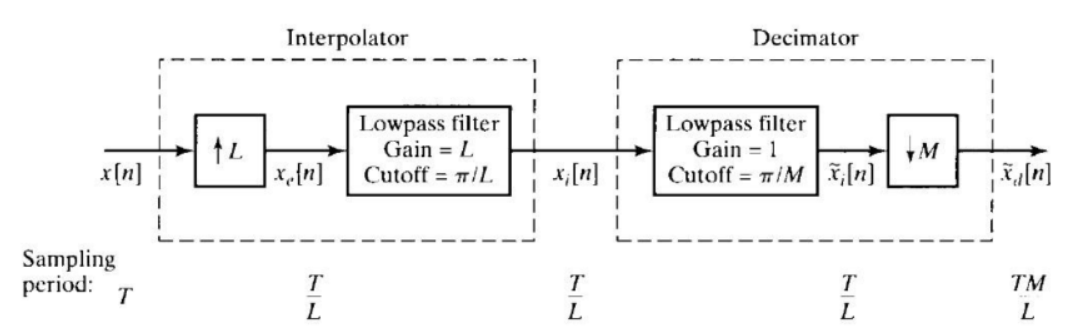
\includegraphics[width=1\textwidth]{/home/jay/Desktop/Dsp-lab/Experiment-8/codes/Q.png}
  \caption{Block Diagram}
\end{figure}
\section{Theory}
\subsection{Interpolation}.
 \begin{itemize}[label=$\bullet$]
	\item Interpolation is a technique used to increase the sampling rate of a discrete-time signal. It involves inserting additional samples between existing samples of a signal to achieve a higher sampling rate.
	\item Interpolation is followed by filtering to remove unwanted frequency components that are introduced during the upsampling process.    
	\item The main purpose of interpolation is to raise the sampling rate at the output of a system, enabling compatibility with another system that requires a higher sampling rate for input.(Example - Changing resolution of image.) 
	\item Interpolation requires upscaling, allowing interpolation only by integer factors. Fractional factors are not feasible for interpolation alone. However, combining interpolation with decimation can achieve an overall rational factor for resampling.
  \end{itemize}
\begin{figure}[ht] % 'h' specifies here (at the current location)
  \centering
  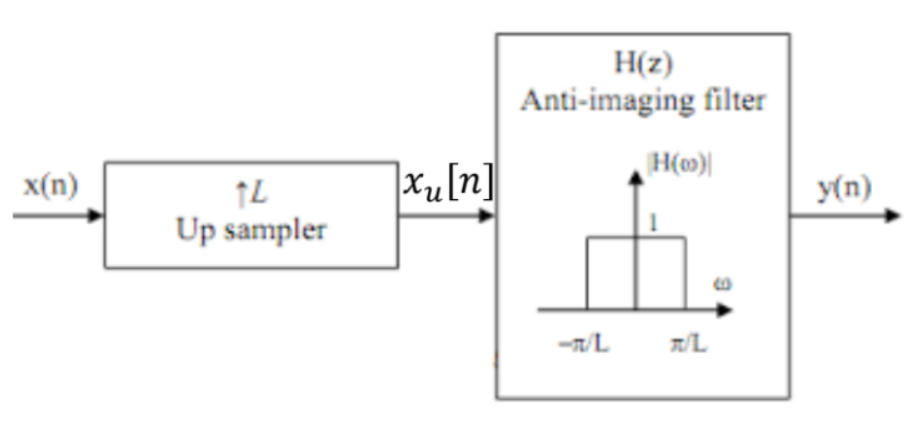
\includegraphics[width=0.5\textwidth]{/home/jay/Desktop/Dsp-lab/Experiment-8/codes/1.png}
  \caption{Practical Interpolator}
\end{figure}
\subsection{Decimation}
\begin{itemize}[label=$\bullet$]
\item Decimation is a process used to reduce the sampling frequency of a discrete-time signal. It involves decreasing the number of samples in the signal to achieve a lower sampling rate.
\item The main purpose of decimation is to conserve computational resources and reduce data storage requirements by lowering the sampling rate of the signal. (for example, data compression, and telecommunications by reducing the amount of data without significant loss of information.)
\item \textbf{Filtering Before down-sampling}, a lowpass filter is applied to the signal to remove high-frequency components above the desired Nyquist frequency of the down-sampled signal.After filtering, the signal is down-sampled.The filter in decimation is crucial to prevent aliasing, ensuring that no frequency components above half the new sampling rate (Nyquist frequency) remain in the down-sampled signal.
\item Decimation is complementary to interpolation, which is used to increase the sampling rate of a signal. Combining decimation with interpolation can achieve arbitrary resampling rates efficiently.
\end{itemize}
\begin{figure}[ht] % 'h' specifies here (at the current location)
  \centering
  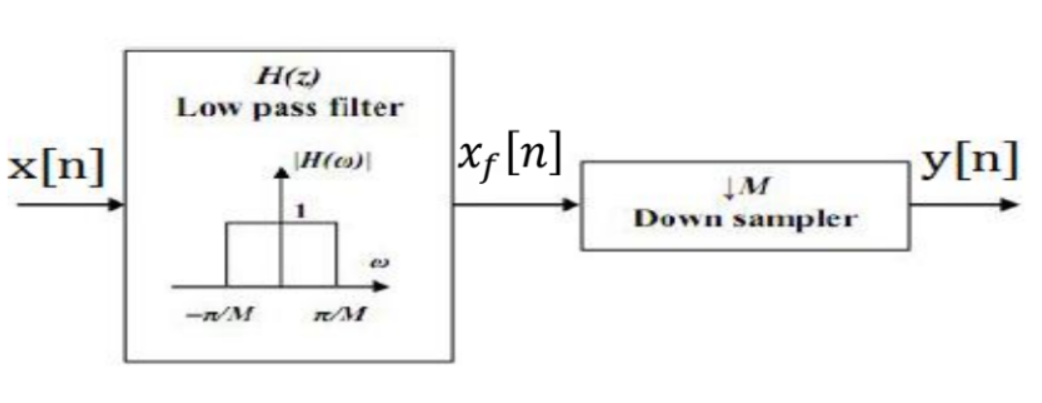
\includegraphics[width=0.5\textwidth]{/home/jay/Desktop/Dsp-lab/Experiment-8/codes/2.png}
  \caption{Practical Decimator}
\end{figure}
\section{How filter cutoff frequencies are decided in Interpolation and Decimation}
\subsection{Interpolation}
\begin{itemize}
    \item The pupose of Interpolation increases the sampling rate of a signal by inserting new samples between existing ones.
    \item When performing interpolation, a low-pass filter is typically used before upsampling to remove high-frequency components that could cause aliasing during the subsequent interpolation process.
    \item The cutoff frequency of the low-pass filter in interpolation is chosen based on the desired new sampling rate after interpolation. It should be set below half of the original sampling rate (Nyquist frequency) to avoid aliasing when new samples are inserted. Specifically, for interpolation by a factor of \( L \) (where \( L \) is an integer greater than 1), the cutoff frequency of the low-pass filter is often set at \(f_c = \frac{f_s}{2L} \), where \( f_s \) is the original sampling frequency.
\end{itemize}
\subsection{Decimation}
\begin{itemize}
    \item The objective of Decimation reduces the sampling rate of a signal by selecting a subset of existing samples.
    \item In decimation, a low-pass filter is applied after downsampling to remove high-frequency components introduced by the downsampling process.
    \item The cutoff frequency of the low-pass filter in decimation is crucial for preventing aliasing in the downsampled signal. The filter's cutoff frequency is typically set at or below \(f_c =  \frac{f_s}{2M} \), where \( M \) is the decimation factor (an integer greater than 1) and \( f_s \) is the original sampling frequency. This ensures that any high-frequency components introduced during downsampling (due to folding) are adequately filtered out.
\end{itemize}

In summary,the choice of filter cutoff frequency is guided by the Nyquist criterion to prevent aliasing. The specific values for these cutoff frequencies are determined by the desired resampling factors relative to the original sampling rate.
\section{MATLAB Simulation}
\subsection{Matlab Code}
This is the main matlab code,
\lstinputlisting[language=Matlab]{/home/jay/Desktop/Dsp-lab/Experiment-8/codes/main.m}
\subsection{Outputs}

\begin{figure}[ht] % 'h' specifies here (at the current location)
  \centering
  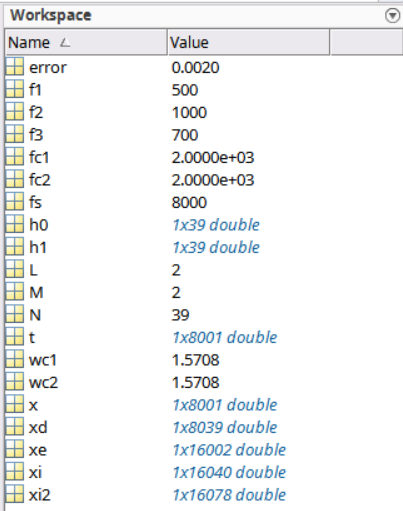
\includegraphics[width=0.4\textwidth]{/home/jay/Desktop/Dsp-lab/Experiment-8/codes/workspace.png}
  \caption{No of samples x(n) is 8001, $x_e(n)$ = L $\times$ 8001, $x_i(n)$  L $\times$ 8001 , $\widetilde{x_i} \approx$ L $\times$ 8001, $\widetilde{x_d} \approx \frac{M}{L} \times$ 8001 samples, (L = M = 2 )}
\end{figure}
\begin{figure}[ht] % 'h' specifies here (at the current location)
  \centering
  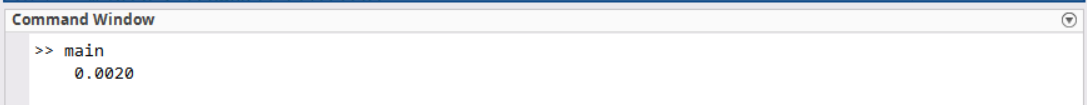
\includegraphics[width=1\textwidth]{/home/jay/Desktop/Dsp-lab/Experiment-8/codes/cmd.png}
  \caption{Mean absolute error for Sampling frequency = 8000Hz}
\end{figure}
\clearpage
\section{Observations}
\begin{enumerate}
    \item \textbf{Upsampling (Interpolation):}
    \begin{itemize}
        \item After upsampling the signal by a factor of 2, the number of samples in the signal increased accordingly (from 8001 to 16002 samples in this case).
        \item The interpolation process involved applying a low-pass filter with a gain of 2 and a cutoff frequency of \( \frac{\pi}{2} \) to remove high-frequency components that could cause aliasing during upsampling.
    \end{itemize}
    
    \item \textbf{Downsampling (Decimation):}
    \begin{itemize}
        \item Following interpolation, the signal was then downsampled by a factor of 2.
        \item A low-pass filter with a gain of 1 and a cutoff frequency of \( \frac{\pi}{2} \) was used after downsampling to eliminate any high-frequency components introduced by the downsampling process.
    \end{itemize}
    
    \item \textbf{Mean Absolute Error:}
    \begin{itemize}
        \item The mean absolute error \( E[|\widetilde{x_d}(n) - x(n)|] \) was calculated to quantify the deviation between the interpolated and original signals which came as 0.002 at fs = 8000Hz and N = 39. This make sense because we have take good enough value of sampling frequecny (i.e  $> 2\times f_{max}$).
        \item This error metric helps assess the accuracy of the resampling process and the effectiveness of the filtering techniques employed.
    \end{itemize}
\end{enumerate}
\section{Conclusion}
\begin{itemize}
    \item \textbf{Interpolation} effectively increased the sampling rate of the input signal by inserting new samples between existing ones. The use of a low-pass filter with an appropriate cutoff frequency helped prevent aliasing during upsampling.
    
    \item \textbf{Decimation} reduced the sampling rate of the signal while maintaining essential signal characteristics. The application of a low-pass filter post-downsampling ensured that unwanted frequency components were adequately filtered out.
    
    \item The overall resampling process, combining interpolation and decimation, allowed for the transformation of the input signal to a different sampling rate, demonstrating the utility of these techniques in applications of telecommunication, image and audio processing.
    
    \item The mean absolute error analysis provided insights into the fidelity of the resampled signal compared to the original, highlighting the importance of proper filtering in maintaining signal integrity during sampling rate conversion.
\end{itemize}

In conclusion, the experiment successfully showcased the principles of interpolation and decimation in signal processing, emphasizing the critical role of filtering in ensuring accurate resampling operations.

\section*{END OF REPORT}
\end{document}
